\documentclass{ieeeaccess}
\usepackage{amsmath}
\usepackage{array}
\usepackage[normalem]{ulem}
\usepackage{ulem}
\usepackage{longtable}
\usepackage{rotating}
\usepackage{multirow}
\usepackage{bm}
\usepackage{epstopdf}
\usepackage{float}
\usepackage{flushend}
\usepackage{amsfonts}
\usepackage{caption}
\usepackage{enumitem}
\usepackage{supertabular}
\usepackage{graphicx}
\usepackage{subfigure}
\usepackage{tabularx}
\usepackage{graphicx}
\usepackage{booktabs}
\usepackage{amssymb}
\usepackage{tabularx}
\usepackage{subfigure}
\usepackage{epstopdf}
\usepackage{algorithmic}
\usepackage{algorithm} %format of the algorithm
\usepackage{amsmath, mathtools}
\usepackage{pifont}
\usepackage{bm}
\usepackage{cases}
\usepackage{flushend}
\usepackage{epsfig}
\def\BibTeX{{\rm B\kern-.05em{\sc i\kern-.025em b}\kern-.08em
    T\kern-.1667em\lower.7ex\hbox{E}\kern-.125emX}}
\begin{document}
\history{Date of publication xxxx 00, 0000, date of current version xxxx 00, 0000.}
\doi{10.1109/ACCESS.2018.DOI}

\title{Efficient Low Rank Regression Based on Nuclear Norm Regularization}
\author{\uppercase{LinLu Wu}\authorrefmark{1},
           \uppercase{Xiangdong Zhang}\authorrefmark{1},
           \uppercase{QianQian Wang}\authorrefmark{1},
           \uppercase{QuanXue Gao}\authorrefmark{1}
}
%\uppercase{Jin Li}\authorrefmark{2},
%\uppercase{Jane YOU}\authorrefmark{3}}
\address[1]{State Key Laboratory of Integrated Services Networks, Xidian University, Xi'an 710071, China}
%\address[2]{School of Software Engineering, Shenzhen Institute of Information Technology, 710071, Shenzhen, Guangdong, China (e-mail: qlinshenz@163.com)}
%\address[2]{The State Key Laboratory of Integrated Services Networks, Xidian University, 710071, Xi'an, China (e-mail: 610887187@qq.com)}
%\address[3]{Department of computing the Hongkong Polytechnique University, Hongkong, China}
%\tfootnote{This paragraph of the first footnote will contain support
%information, including sponsor and financial support acknowledgment. For
%example, ``This work was supported in part by the U.S. Department of
%Commerce under Grant BS123456.''}
%\markboth
%{Author \headeretal: Preparation of Papers for IEEE TRANSACTIONS and JOURNALS}
%{Author \headeretal: Preparation of Papers for IEEE TRANSACTIONS and JOURNALS}
\corresp{Corresponding author: Xiangdong Zhang (e-mail: xdchen@mail.xidian.edu.cn), QianQian Wang(qianqian174@foxmail.com).}

\begin{abstract}
In real world application, data often has a low rank structure as it contains much redundant information, such as face image. Low rank regression method has been proved to be an effective learning mechanism by exploring the low rank structure of the real world data. However, the majority of the existing low rank regression methods just impose the low rank constraint on the coefficient matrix so that they do not take into account the global information of the data. In addition, those methods need much computing time, especially when the data dimension is high. In this paper, we proposed a novel model called Nuclear Norm Low Rank Regression (NNLR) which directly imposes low rank constraint on projected data. In this way, our method can preserve the global geometric structure of data and obtain an explicit solution. An efficient iterative algorithm is proposed to solve the optimize problem. Moreover, we extend the application of NNLR from single view data to multi-view data. Extensive experiments on some well-known datasets containing single-view and multi-view datasets show that NNLR is superior to existing low rank regression method.
\end{abstract}

\begin{keywords}
Low rank regression, Nuclear norm, Efficient solution
\end{keywords}

\titlepgskip=-15pt

\maketitle

\section{Introduction}
\IEEEPARstart{M}{ultivariable} linear regression is a basic and effective technique in data mining and machine learning. It models the relationship between predictors and responses by a linear approach. Ridge regression can achieve better results by adding a Frobenius norm based regularization on linear regression loss objective~\cite{ref20,ref21}. Other classical methods include lasso regression~\cite{ref22}, least angle regression~\cite{ref23}, and elastic net regression~\cite{ref24}.

In many applications, such as gene expression, document classification and face recognition, predictor and response are high dimensional, the performance of linear regression methods may degrade when deal with this kind of data. The reason may be that the ordinary linear regression method is equivalent to separately regressing each response on the set of predictors, which ignores the underlying correlations between responses and that may be infeasible in the case of high-dimension. In general, the curse-of-dimensional can be mitigated by dimension reduction.

An efficient mechanism to solve the problem of curse-of-dimensional in linear regression method is low rank regression, which means the rank of the coefficient matrix is less than both the dimension of predictor and response. In low rank regression method, dimension reduction is achieved by imposing low rank constraint on the coefficient matrix. Anderson first introduced the low rank regression in~\cite{ref01}. Later many related literature, such as~\cite{ref07,ref12,ref14}, were proposed. For more description and discussion of reduced-rank regression, we refer the reader to the books~\cite{ref30,ref31}. All these works can be roughly divided into two categories.

The first category is rank regularization methods, which can be viewed as a L0-norm regularizer in terms of the singular value vector of the coefficient matrix. The rank regularization was first proposed in~\cite{ref27}. Adding a ridge regularization was proposed in~\cite{ref26}. Although the general rank minimization is a non-convex and NP-hard problem, the objectives with rank regularization are solvable in~\cite{ref07} by using the singular value shrinkage estimator. After that, Cai et al.~\cite{ref11} introduced a low rank regression method named low rank ridge regression (LRRR), and they solved the problem by expressing the coefficient matrix as the product of two lower rank matrices. Then, Zheng et al.~\cite{ref12} extended the low rank regression method to a multi-view low rank regression method and provided a closed form solution. ~\cite{ref28} solved the problem when the responses have a tensor structure. But the discontinuity of rank in rank regularization method results in inflexible bias-variance trade-off in model fitting of application.

The second category is nuclear norm regularization methods, which can also be viewed as a L1-norm of the singular value vector of the coefficient matrix. Nuclear norm based methods are a hot topic of research in recent years, such as~\cite{ref28,ref29} which introduced nuclear norm based regression models as classifiers used in face recognition. Yuan et al.~\cite{ref02} proposed a nuclear norm regularization regression(NNRR) method, in which the regularizer is defined as the nuclear norm of the coefficient matrix. The solution of the nuclear norm method can be found in~\cite{ref03,ref14}, from which we can find that the solution is computationally intensive. As we know, by adding a ridge regularization~\cite{ref04} on the linear regression loss function, i.e. ridge regression, can achieve better performance than linear regression, It is regrettable that the method in~\cite{ref02} did not consider this point.

More recently, low-rank robust regression (denoted as LR-RR)~\cite{ref33} has been proposed to learn a robust regression model in the clean low-rank sample space highly correlated to output variables. Although LR-RR can reduce most arbitrary sparse outliers/noise both within the domain subspace and outside of it, it tends to be sensitive to outliers/noise among a set of disjoint subspaces. Then, Zhang et al.~\cite{ref32} proposed low-rank-sparse representation for robust regression(LRS-RR) which can handle the outliers/noise lying on the sparsely disjoint subspaces. Moreover, Li et al.~\cite{ref34} proposed a low rank Extreme learning Machine(LR-ELM) method. ELM is a least-square based learning algorithm and LR-ELM captures the underlying relationship between features and preserves the global geometric structure by imposing low-rank constraints with the extracted features.

However, those work improves the performance of linear regression by imposing low rank constraint on the coefficient matrix, they do not take into account the global information of projected data. In addition, they need much computing-time especially for high dimensional data. To tackle these problems, in this paper, we propose a new nuclear norm linear regression method (NNLR). We compared our method with other similar methods in Table ~\ref{tab8}, and the contributions of this paper are summarized as follows:


\begin{itemize}
  \item Firstly, we impose low rank constraint on the projected data which means the product of the data matrix and the coefficient matrix rather than the coefficient matrix. This set-up can preserve the global geometric structure of data while imposing low rank constraint on coefficient. Another advantage of this set-up is the optimize problem can be solved efficiently.
  \item Secondly, our method includes a ridge regularization which makes the method more robust ~\cite{ref19,ref25}. Therefore, NNLR allows the low rank regression problem to be solved stably and efficiently. Compared to the discontinuous rank regularization methods, our method results flexible bias-variance trade-off in the model fitting. Compared to the computationally intensive nuclear norm method introduced in Yuan et at.~\cite{ref02}, our method is more robust and efficient.
  \item Thirdly, we developed an efficient iterative algorithm to solve NNLR. The proposed optimizer algorithm consumes little training time, especially when the data dimension is high.
  \item Finally, we extended the NNLR method to multi-view case in which the result is decided by the sum of each view. Extensive experiment on some well-known datasets shows that NNLR outperforms LRRR and other related method.
\end{itemize}
\begin{table}[t]
\renewcommand\arraystretch{1.3}
\newcommand{\bb}[1]{\raisebox{0pt}[0pt][0pt]{\shortstack{#1}}}
\newcommand{\PreserveBackslash}[1]{\let\temp=\\#1\let\\=\temp}
\newcommand{\tabincell}[2]{\begin{tabular}{@{}#1@{}}#2\end{tabular}}
\newcolumntype{C}[1]{>{\PreserveBackslash\centering}p{#1}}
\newcolumntype{R}[1]{>{\PreserveBackslash\raggedleft}p{#1}}
\newcolumntype{L}[1]{>{\PreserveBackslash\raggedright}p{#1}}
\caption{ Comparison with related methods.}\label{tab8}
\vspace{-2mm}
\begin{center}
\begin{tabular}
{
C{40pt}
%|@{\extracolsep{0.7pt}}C{60pt}@{\extracolsep{1pt}}
%|@{\extracolsep{0.7pt}}C{60pt}@{\extracolsep{1pt}}
|@{\extracolsep{0.7pt}}L{95pt}@{\extracolsep{1pt}}
|@{\extracolsep{0.7pt}}L{95pt}@{\extracolsep{1pt}}
}
\toprule
Methods& Advantage & Disadvantage \\
\hline
NNRR ~\cite{ref02}&(1) Capture the underlying correlations between responses.& (1) Computationally intensive.
\quad\quad\quad\quad\quad\quad\quad(2) Poor robustness.\\
 \hline
LRRR~\cite{ref11} & (1) Capture the underlying correlations between responses.\quad \quad\quad\quad\quad\quad\quad(2) Include L2-regularizer. & (1) Inflexible bias-variance trade-off in model fitting. \quad  (2) Computationally intensive when dimension is high.\\
 \hline
 LR-RR~\cite{ref33} & (1) Robust to noise. & (1) Neglect the underlying correlations between responses.\\
 \hline
NNLR & (1) Capture the underlying correlations between responses. \quad\quad\quad\quad\quad\quad\quad(2) Preserve the global geometric structure.  \quad\quad\quad(3) Include L2-regularizer. & (1) Two continuous parameters need to adjust.\\
\hline
\toprule
\end{tabular}
\end{center}
\vspace{-6mm}
\end{table}


%\section{Introduction of 2DPCA and 2DPCA-L1}
\section{Background}

Multi-variable linear regression is a basic regression method due to it is simple and effective in data mining and machine learning. Suppose there are $n$ observations, response ${y_i} \in {R^c}$ and predictor ${x_i} \in {R^p}$, the multi-variable linear regression model
\begin{equation}\label{eq01}
Y = {X^T}C  + E
\end{equation}
\noindent where indicator matrix $Y = [{y_1},{y_2},...,{y_n}]^T$ and data matrix $X = [{x_1},{x_2},...,{x_n}]$, $C  \in {R^{p \times c}}$ is a coefficient matrix, $E$ is the regression noise. To solve this problem, Ordinary least squares approach assumes a linear dependence among responses and boils down to finding a matrix $C$ that minimizes the squared error $\left\| {Y - {X^T}C {\rm{ }}} \right\|_F^2$. But this method usually have low performance in the high-dimension case as it ignores the underlying correlations between responses(classes) and which can be mitigated by dimension reduction. In ~\cite{ref11}, we can see that low rank regression is equivalent to perform Linear Discriminant Analysis (LDA) and linear regression simultaneously. In low rank regression method, dimension reduction is achieved by imposing low rank constraint on the coefficient matrix.

To improve the performance of linear regression method, in recent work~\cite{ref11} researchers introduced a method named low rank ridge regression (LRRR), which is shown in following
\begin{equation}\label{eq02}
\left\| {Y - {X^T}AB} \right\|_F^2 + \lambda \left\| {AB} \right\|_F^2
\end{equation}
where ${\left\| {} \right\|_F}$ denotes the Frobenius norm, $A \in {R^{p \times s}}$, $B \in {R^{s \times c}}$ and $s < \min (p,c)$, $s$ is the rank of $C$ and $\lambda$ is the nonnegative parameter. Similarly, we can see that the LRRR objective function is equivalent to the following problem
\begin{equation}\label{eq20}
\left\| {Y - {X^T}C } \right\|_F^2 + \lambda \left\| C  \right\|_F^2 \qquad  s.t. \quad rank(C ) \le s
\end{equation}

Therefore, we can see LRRR is a robust rank regularization method. Because rank is discontinuity, i.e. $s$ can only take a finite number of integers, LRRR results in an inflexible bias-variance trade-off in the model fitting. Fortunately, nuclear norm regularization regression methods result in a continuous solution path. A nuclear norm regularization method introduced in ~\cite{ref02} is shown in following
\begin{equation}\label{eq03}
\left\| {Y - {X^T}C } \right\|_F^2 + \lambda {\left\| C  \right\|_*}
\end{equation}
where ${\left\| {} \right\|_*}$ denotes the nuclear norm. The nuclear norm is the L1-norm of the singular value vector which encourages sparsity among the singular values and achieves low rank. The solution to problem (\ref{eq03}) generally does not have an explicit form. Extensive works have been devoted to this minimization problem~\cite{ref03}~\cite{ref11}, but they are computationally intensive for large-scale data. In order to make the method more robust~\cite{ref19,ref25}, we incorporate a ridge regularizer, i.e.$\left\| C  \right\|_F^2$, into our method.

\section{Nuclear norm based low rank regression}

\subsection{Motivation and NNLR Method}

As above analyses, rank regularization results in inflexible bias-variance trade-off in the model fitting, the solution to nuclear norm regularization problem is computationally intensive especially in high dimension case. In addition, both of them do not take into account the global information of data which is important for classification.

According to Sylvester Inequality, we know that the rank of the product of the data matrix and the coefficient matrix smaller than the rank of the coefficient matrix, i.e. $rank({X^T}C ) \le rank(C )$. So we can see that low rank constraint on $C$ impairs low rank constraint on ${X^T}C $ and the converse is not necessarily true. The following theorem introduced in ~\cite{ref18} showed that low rank constraint on ${X^T}C $ is equal to constraint on $C$.

\textbf{Theorem 1}: If $rank({X^T}C ) \le r$ then there is a matrix ${C'}$ with $rank({C'}) \le r$ and ${X^T}{C} = {X^T}{C'}$.

\textbf{Proof:} Suppose $rank({X^T}C ) = {r'} \le r$, we can write ${X^T}C = BA$ where $B \in {R^{(p + 1) \times {r'}}}$ and $A \in {R^{{r'} \times q}}$ with $rank(B) = rank(A) = {r'}$. Since the dimensions of $span\{ BA\} $ (the space spanned by the columns of the matrix ) and $span\{ B\} $ are noth ${r'}$, we have $span\{ B\}  = span\{ BA\}  = span({X^T}C ) \subseteq span\{ {X}\}$ and thus there is a matrix $D$ such that $B = {X^T}D$
This implies ${X^T}C  = {X^T}DA$ and the matrix ${C'}:=DA$ has rank at most ${r'}$ since $rank(A) = {r'}$

To improve low rank regression method, we need to preserve the global geometric structure, i.e. low rank structure, in the subspace.
Therefore we use the nuclear norm of ${X^T}C $ archive the low rank constraint on $C$. There are three advantages of this set-up. First, ${\left\| {{X^T}C } \right\|_*}$ can describe the global geometric structure. of data which is important for classification, but ${\left\| C  \right\|_*}$ can not. Second, supposing $rank({X^T}C ) = a$, according to theorem 1, it is possible that there is a matrix ${C'}$ satisfying $rank({X^T}C ) $<$ a$. In this case, if we impose low rank constraint on the coefficient matrix $C$, we will get an inaccurate solution, but if we impose low rank constraint on ${X^T}C$, the solution will be more explicit. Third, the problem, $\mathop {\min }\limits_C  \left\| {Y - {X^T}C } \right\|_F^2 + \lambda {\left\| {{X^T}C } \right\|_*}$, can be solved more explicitly and efficiently by singular value shrinkage estimator which will be introduce in the next section. Therefore, this set-up can preserve more useful information which may improve the performance and result in a more explicit and efficient solution.

\subsection{Nuclear norm based low rank regression for single-view problem}

As introduced in~\cite{ref19,ref25}, by adding a Frobenius norm based regularization on the linear regression loss, ridge regression can achieve better performance and more robust than linear regression. Therefore, it is important and necessary to add the ridge regularization into low rank regression formulation. In addition, to improve the low rank regression method, we impose the low rank constraint on ${X^T}C $ rather than $C$ for more efficient solution and better performance. So, we propose the following nuclear norm based low rank regression(NNLR) as
\begin{equation}\label{eq04}
\mathop {\min }\limits_C  \left\| {Y - {X^T}C } \right\|_F^2 + {\lambda _1}\left\| C  \right\|_F^2 + {\lambda _2}{\left\| {{X^T}C } \right\|_*}
\end{equation}
where $C  = [{C _1},{C _2},...,{C _n}] \in {R^{p \times c}}$ is the coefficient matrix. ${\lambda _1}$ is the regularization parameter, ${\lambda _2}$ is the positive scalar.

To make the problem easy to solve, Eq. (\ref{eq04}) can be written as
\begin{equation}\label{eq05}
\begin{array}{l}
\mathop {\min }\limits_{C ,M} \left\| {{X^T}C  - Y} \right\|_F^2 +{\lambda _1}\left\| C  \right\|_F^2 + {\lambda _2}{\left\| M \right\|_*},\\
 \;\;\;\;\;\;\;\;\;\;\;\;\;\;\;\;\;\;{\rm s.t.} \; \; \; M={X^T}C,
 \end{array}
\end{equation}



\subsubsection{Iterative solution}

According to Augmented Lagrangian method(ALM) introduced in~\cite{ref13}, we can replace the constrained optimization problem showed in Eq. (\ref{eq05}) by the following unconstrained problem
\begin{equation}\label{eq06}
\begin{array}{l}
\mathop {\min }\limits_{C ,M,A} \left\| {{X^T}C  - Y} \right\|_F^2 + {\lambda _1}\left\| C  \right\|_F^2 + {\lambda _2}{\left\| M \right\|_*}\\ \;\;\;\;\;\;\;\;\;\;\;\;\;\;\;\;+ \displaystyle\frac{\mu }{2}\left\| {\displaystyle\frac{A}{\mu } + M - {X^T}C } \right\|_F^2
\end{array}
\end{equation}
where $\mu$ is a positive scalar, $A$ is an estimate of the Lagrange multiplier. (\ref{eq06}) is a deformation of standrad ALM , and it is  equivalent to the form of standrad ALM when we update M and C and can be solved more convenient.

\textbf{Fix $A$ and $C$, update $M$} When $A$ and $C$ is fixed, the first and second item of problem (\ref{eq06}) could be seen as constant, then the problem in Eq. (\ref{eq06}) transforms into
\begin{equation}\label{eq07}
\mathop {\min }\limits_M {\lambda _2}{\left\| M \right\|_*} + \displaystyle\frac{\mu }{2}\left\| {\frac{A}{\mu } + M - {X^T}C } \right\|_F^2
\end{equation}






To solve this problem, we need the theorem of singular value shrinkage operator ~\cite{ref14}, Consider the singular value decomposition (SVD) of $H \in {R^{m \times n}}$ with rank $r$:
\begin{align}
H = U & \Sigma {V^T}  \qquad  \Sigma=diag({\{{\sigma _i}\} _{1 \le i \le r}})
\end{align}

\makeatletter
\noindent
\def\hlinew#1{%
  \noalign{\ifnum0=`}\fi\hrule \@height #1 \futurelet
   \reserved@a\@xhline}
\makeatother
\vspace{0.3cm}
\begin{tabular}{p{8cm}l}
  \hlinew{1.5pt}
  % after \\: \hline or \cline{col1-col2} \cline{col3-col4} ...
  \textbf{Algorithm 1} Nuclear norm low rank regression\\
  \hline
  \textbf{Input:} Data matrix $X \in {R^{p \times n}}$, regularization weight parameter$\lambda_1$ and $\lambda_2$,  parameter $\rho$, $1.1 \le \rho  \le 1.2$, label matrix $Y \in {R^{n \times c}}$. \\
    \textbf{Repeat:} \\
  Compute the optimal solution $M$ of Eq. (\ref{eq07}) by using Eq. (\ref{eq11}).\\
  Compute the optimal solution $C$ of Eq. (\ref{eq12}) by using Eq. (\ref{eq14}).\\
  Update $A$ and $\mu$ by using rule (\ref{eq15}).\\
  \textbf{Until converge}\\
  \textbf{Output:} Coefficient matrix $C  \in {R^{p \times c}}$.\\
  \hlinew{1.5pt}
\end{tabular}
\noindent where $U \in {R^{m \times r}}$, $V \in {R^{n \times r}}$ and the singular value ${\sigma _i}$ are positive. For each $\tau  \ge 0$
define the singular value shrinkage operator as follows
\begin{equation}\label{eq08}
\begin{array}{l}
{D_\tau }(H): = U{D_\tau }(\Sigma ){V^T} \\
{D_\tau }(\Sigma ) = diag(\max ({\sigma _i} - \tau ,0))
\end{array}
\end{equation}

\textbf{Theorem 2}: For each $\tau  \ge 0$ and $Q \in {R^{m \times n}}$, the singular value shrinkage operator obeys:

\begin{equation}\label{eq09}
{D_\tau }(Q) = \mathop {\arg \min }\limits_H \displaystyle\frac{1}{2}\left\| {H - Q} \right\|_F^2 + \tau {\left\| H \right\|_*}
\end{equation}

Then, the problem in Eq. (\ref{eq07}) can be written as following:
\begin{equation}\label{eq10}
\mathop {\min }\limits_M \displaystyle\frac{1}{2}\left\| {M - \left({X^T}C  - \displaystyle\frac{A}{\mu }\right)} \right\|_F^2 + \displaystyle\frac{{{\lambda _2}}}{\mu }{\left\| M \right\|_*}
\end{equation}

So, $M^*$, the optimal solution to Eq. (\ref{eq07}), can be formed by
\begin{equation}\label{eq11}
{M^*} = {D_\tau }({X^T}C  - \displaystyle\frac{A}{\mu })
\end{equation}

\textbf{Fix $M$ and $A$, update $C$} Since $M$ and $A$ is fixed, the third item of Eq. (\ref{eq06}) can be seen as constant. Therefore, the problem (\ref{eq06}) becomes
\begin{equation}\label{eq12}
\mathop {\min }\limits_C  \left\| {{X^T}C  - Y} \right\|_F^2 + {\lambda _1}\left\| C  \right\|_F^2 + \displaystyle\frac{\mu }{2}\left\| {\displaystyle\frac{A}{\mu } + M - {X^T}C } \right\|_F^2
\end{equation}

Let $J(C )$ be the object function of problem in Eq. (\ref{eq12}), Taking derivative of $J$ w.r.t. $C$, we have
\begin{equation}\label{eq13}
\frac{{\partial J}}{{\partial C }} = [(2 + \mu ){X^T}X + 2{\lambda _1}I]C  - {X^T}(2Y + \mu M - A)
\end{equation}
where $I \in {R^{n \times n}}$ is an identity matrix. Setting Eq. (\ref{eq13}) to zero, the optimal solution to the problem (\ref{eq12}) can be written as follows
\begin{equation}\label{eq14}
{C ^*} = {[(2 + \mu ){X^T}X + 2{\lambda _1}I]^{ - 1}}{X^T}(2Y + \mu M - A)
\end{equation}


\textbf{Fix $M$ and $C$, update $A$}According to Augmented Lagrangian method, the variable matrix $A$ and coefficient $\mu$ can be updated by the following rule
\begin{equation}\label{eq15}
A \leftarrow A + \mu (M - {X^T}C )  \qquad  \mu  \leftarrow \rho \mu
\end{equation}
where $\rho$ is a constant which is between 1.1 and 1.2 empirically. \\

\vspace{2mm}
\makeatletter
\noindent
\def\hlinew#1{%
  \noalign{\ifnum0=`}\fi\hrule \@height #1 \futurelet
   \reserved@a\@xhline}
\makeatother
\begin{tabular}{p{8cm}l}
  \hlinew{1.5pt}
  % after \\: \hline or \cline{col1-col2} \cline{col3-col4} ...
  \textbf{Algorithm 2}  Multi-view low rank regression \\
  \hline
  \textbf{Input:} Data matrix ${X_v} \in {R^{{p_v} \times n}}$, $v = 1,2,...,V$ regularization weight parameter$\lambda_1$ and $\lambda_2$, parameter $\rho$, $1.1 \le \rho  \le 1.2$, label matrix  $Y \in {R^{n \times c}}$. \\
    \textbf{For view $v$:} \\

  Calculate coefficient matrix of each view$C_v$ by Algorithm 1.\\
  \textbf{end}\\
  \textbf{Output:} Coefficient matrix of each view $C_v  \in {R^{p_v \times c}}$, $v = 1,2,...,V$. \\
  \hlinew{1.5pt}
\end{tabular}


\subsubsection{Algorithm}

We present Algorithm 1 to sum up the steps of nuclear norm low rank regression model for single-view problem. The input of the algorithm are data matrix $X \in {R^{p \times n}}$ which is centered and normalized, where $P$ is the dimension of data and $N$ is the number of sample, class label indicator matrix $Y \in {R^{n \times c}}$, where $C$ is the number of class, the regularization weight parameter$\lambda_1$, the parameter of nuclear norm item and the parameter of Augment Lagrange method. The output of this algorithm is matrix $C  \in {R^{p \times c}}$. We need to repeat updating the variable in Eq. (\ref{eq06}) until the result of Eq. (\ref{eq06}) converge, and then we get the optimal solution $C^*$.

For single-view situation, after getting optimal solution, the following decision function is used to decide the class of sample $x$
\begin{equation}\label{eq16}
\mathop {\arg \max }\limits_{1 \le j \le c} {(y)_j}
\end{equation}
where vector $y = {x^T}{C ^*} \in {R^{1 \times c}}$, ${(y)_j}$ is the $j$-th element of $y$. The classification of sample $x$ corresponds to the index of maximum value in vector $y$.

\subsubsection{Computational complexity of NNLR}

In the iterations of NNLR, the computational costs are mainly SVD, eigen decomposition and matrix multiplication. For the data matrix $X \in {R^{p \times n}}$, the computation complexity of full SVD is $o(p*{n^2})$. Each iteration of NNLR mainly includes the SVD of ${X^T}C$, so the computational cost is $o(n*{c^2})$. In general, $c$ is is a small value and so the solution is efficient.  In addition, we need to compute the covariance matrix ${X^T}X$, which is up to $o(p*{n^2})$ in each iteration, and then we need to do eigen decomposition,which needs $o({n^3})$. Hence, the total complexity for NNLR is $o(p*{c^2} + p*{n^2} + {n^3})$ and $t$ s the iteration number.



\subsection{Nuclear norm based low rank regression for multi-view problem}

In many tasks~\cite{ref36,ref37,ref38}, the data include information from many views. Therefore, our method should be extended to work for multi-view problem. When the data includes many views, the objective function becomes
\begin{equation}\label{eq17}
\mathop {\min }\limits_C  \sum\nolimits_v {\{ \left\| {Y - X_v^T{C _v}} \right\|_F^2 + {\lambda _1}\left\| {{C _v}} \right\|_F^2 + {\lambda _2}{{\left\| {X_v^T{C _v}} \right\|}_*}\} }
\end{equation}
where ${X_v} \in {R^{{p_v} \times n}}$, ${C _v} \in {R^{{p_v} \times c}}$, ${p_v}$ is the dimension of view $v$, $\sum\nolimits_v {{p_v}}  = p$, $v = 1,2,...,V$.

\begin{figure*}[!t]
  \centering
  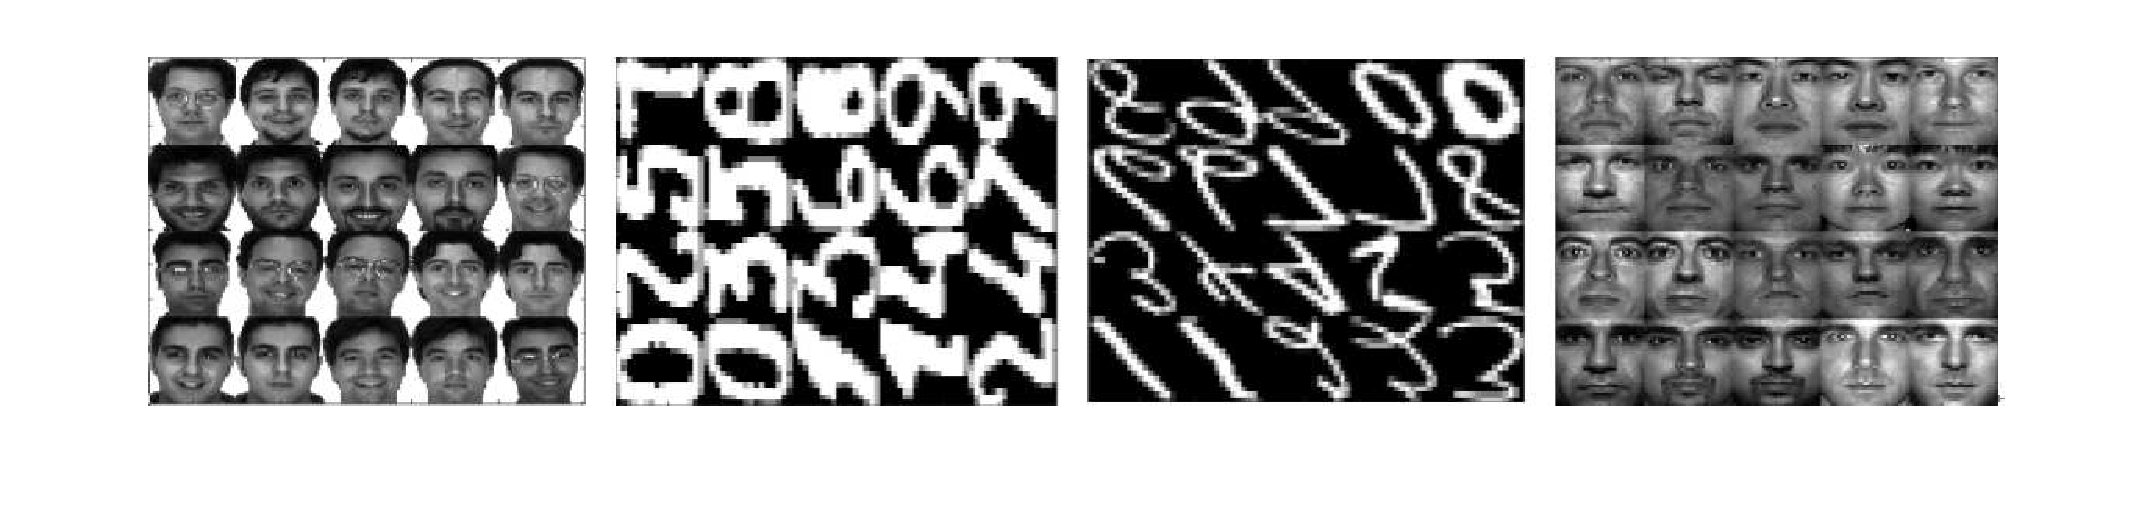
\includegraphics[width=16cm]{dataset}
  \caption{Some samples from AR, Digits, USPS and Extended Yale B.}\label{fig1}
\end{figure*}

In multi-view case, we predict a class of sample $x$ using algorithm 1 for each view and then obtain the ${C _v}$ of each view. Then, we learn label vector $y \in {R^{1 \times c}}$ that minimizes the difference between itself and projected data of each view $x_v^T{C _v}$
\begin{equation}\label{eq18}
\mathop {\min }\limits_y \sum\nolimits_v {\left\| {x_v^T{C _v} - y} \right\|} _F^2
\end{equation}


The optimum solution of Eq. (\ref{eq18}) be shown as
\begin{equation}\label{eq19}
y = \left( {\sum\nolimits_v {x_v^T} {C _v}} \right)/V
\end{equation}

After obtaining $y$, we can get the class indicator of sample $x$ by using Eq. (\ref{eq16}). The Algorithm to solve multi-view low rank regression problem is described in Algorithm 2.



\section{Experiments}

In this section, we perform experiments on 4 different datasets including single-view data and multi-view-data. We compare the recognition rate of NNLR with the classical method and related methods which are rank regularized low rank regression method LRRR, sparse regression based on L21 norm method L21LR, ridge regression RR and linear regression LR. In addition, as suggested by referees, we compare our method with two new methods, LR-RR~\cite{ref32} and LR-ELM~\cite{ref34}. The solution to these methods in multi-view case is similar to the method introduced in section 3.3, i.e. we calculate the coefficient matrix of each view separately and then get the last result of classification by Eq. (\ref{eq19}) and Eq. (\ref{eq16}).

\begin{table}[!t]
\renewcommand\arraystretch{1.3}
\newcommand{\bb}[1]{\raisebox{0pt}[0pt][0pt]{\shortstack{#1}}}
\newcommand{\PreserveBackslash}[1]{\let\temp=\\#1\let\\=\temp}
\newcolumntype{C}[1]{>{\PreserveBackslash\centering}p{#1}}
\newcolumntype{R}[1]{>{\PreserveBackslash\raggedleft}p{#1}}
\newcolumntype{L}[1]{>{\PreserveBackslash\raggedright}p{#1}}
\caption{ The summary of the single-view datasets.}\label{tab5}
\begin{center}
\begin{tabular}
{
C{60pt}
%|@{\extracolsep{0.7pt}}C{60pt}@{\extracolsep{1pt}}
%|@{\extracolsep{0.7pt}}C{60pt}@{\extracolsep{1pt}}
%|@{\extracolsep{0.7pt}}C{60pt}@{\extracolsep{1pt}}
|@{\extracolsep{0.7pt}}C{50pt}@{\extracolsep{1pt}}
|@{\extracolsep{0.7pt}}C{50pt}@{\extracolsep{1pt}}
|@{\extracolsep{0.7pt}}C{50pt}@{\extracolsep{1pt}}}
\toprule
 Dataset& $n$ &$c$ & $d$ \\
\hline
AR& 1680 & 12 & 2000 \\
 \hline
Extended Yale B & 1984 & 31 & 1024\\
 \hline
Cal101-HOG & 441 & 7 & 620 \\
 \hline
Cal101-LBP & 441 & 7 & 1160 \\
 \hline
Cal101-Sift & 441 & 7 & 2560\\
\toprule
\end{tabular}
\end{center}
\end{table}



\subsection{Details of Datasets}

Extended Yale B face dataset includes 1984 frontal-face pictures of 31 people with different lighting conditions dataset, where each person has 64 pictures and the size of each picture is $32 \times 32$.

A subset of the AR face dataset~\cite{ref15} containing 1680 images from 12 individuals were selected and used in our experiments. The pixel values were normalized on 0-255 and the size of images is 50 rows and 40 columns.

USPS Handwrite Digits contain 10 classes, 0 through 9, and each class has 1100 images which is 8 bit gray image. We randomly select 110 images from each class for our single-view experiment.

MSRC~\cite{ref16}is an image scene data including trees, buildings, planes, cows, faces, cars and so on. It has 210 images from 7 classes and every class has 30 images. We extract 5 features from the original picture making up new dataset for our multi-view experiment.

Digits consists of the features of handwritten numbers (0-9) extracted from the Netherlands utility graph collection. Each number (category) digitized in the binary image has 200 examples that are represented in the six feature sets (views) in this data set. View-1 is a feature set of 76 Fourier coefficients of the character shapes; View-2 is a featureset of 216 profile correlations; View-3 is a feature set of 64 Karhunen-Love coefficients; View-4 is a feature set of 240 pixel averages in a $2 \times 3$ window; View-5 is a feature set of 47 Zernike moments; View-6 is a feature set of 6 Morphological features.

The Caltech101 database is a dataset with 101 image classes. In our experiments, we selected seven of these classes, namely Face, Dolla-Bill, Garfield, Motorbikes, Stop-Sign, Snoopy and Windsor-Chair, a total of 441 image. Then, we extract three features from each image. View-1 is a Cal101-HOG feature of 620 dimensions, view-2 is an 1160-dimensional Cal101-LBP feature and view-3 is a 2560-dimensional Cal101-Sift feature. We use the 3 features separately in the single-view experiment and  sets (Cal101-HOG, Cal101-LBP) and (Cal101-HOG, Cal101-LBP, Cal101-Sift) in the multi-view experiments.

Some sample images are shown in FIGURE \ref{fig1}.

\begin{table}[t]
\renewcommand\arraystretch{1.3}
\newcommand{\bb}[1]{\raisebox{0pt}[0pt][0pt]{\shortstack{#1}}}
\newcommand{\PreserveBackslash}[1]{\let\temp=\\#1\let\\=\temp}
\newcolumntype{C}[1]{>{\PreserveBackslash\centering}p{#1}}
\newcolumntype{R}[1]{>{\PreserveBackslash\raggedleft}p{#1}}
\newcolumntype{L}[1]{>{\PreserveBackslash\raggedright}p{#1}}
\caption{ The summary of the multi-view datasets.}\label{tab6}
\begin{center}
\begin{tabular}
{
C{70pt}
%|@{\extracolsep{0.7pt}}C{60pt}@{\extracolsep{1pt}}
%|@{\extracolsep{0.7pt}}C{60pt}@{\extracolsep{1pt}}
|@{\extracolsep{0.7pt}}C{25pt}@{\extracolsep{1pt}}
|@{\extracolsep{0.7pt}}C{25pt}@{\extracolsep{1pt}}
|@{\extracolsep{0.7pt}}C{25pt}@{\extracolsep{1pt}}
|@{\extracolsep{0.7pt}}C{75pt}@{\extracolsep{1pt}}}
\toprule
Dataset& $n$ & $c$ & $v$ & $d_v$ \\
\hline
MSRC&210&7&5&24,576,512,256,254\\
 \hline
Cal101&441&7&3&620,1160,2560\\
 \hline
Cal101-HOG\&LBP &441&7&2&620,1160\\
 \hline
Digits & 2000 &10 &6 & 76,216,64,240,47,6\\
\toprule
\end{tabular}
\end{center}
\end{table}

\subsection{Single-view Experiments}

In the single-view experiments, we choose AR, PIE, USPS and features of cal101 dataset to complete the experiment. In order to show the influence of dimensions on the efficiency of the algorithm, we separately use the Cal101-HOG, Cal101-LBP and Cal101-Sift in experiments. For AR, PIE and USPS, 50\% images of each individual randomly selected are used as the training set and the rest as the testing set. Summary of the single-view datasets attributes are presented in TABLE \ref{tab5}, where $n$ is sample number, $c$ is class number, $d$ is the dimension of features. For the cal101 dataset, we randomly select 290 images for training and the rest for test. For all the experiments, we average the results over 10 random splits. We also computed the training time (in seconds) of all the methods on the datasets used in the experiments. All the experiments were run on a PC (CPU: Intel Core i7-4790, 3.6 GHz; RAM: 16 GB; 64-bit operation system).

FIGURE \ref{fig2} shows the recognition rate histogram, TABLE \ref{tab1} shows the mean and standard deviation of the accuracy over 10 random split. TABLE \ref{tab2} describes the mean and standard deviation of computing time.



\begin{figure}[t]
  \centering
  % Requires \usepackage{graphicx}
  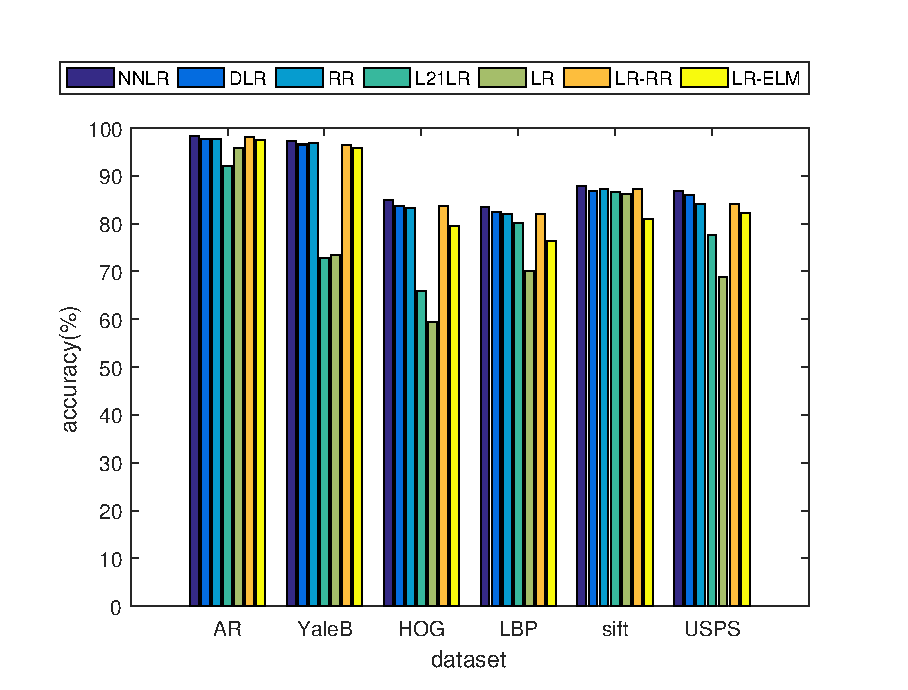
\includegraphics[width=8cm]{single_view}\\
  \caption{Recognition rate of single-view datasets.}\label{fig2}
\end{figure}

\begin{figure}[t]
  \centering
  % Requires \usepackage{graphicx}
  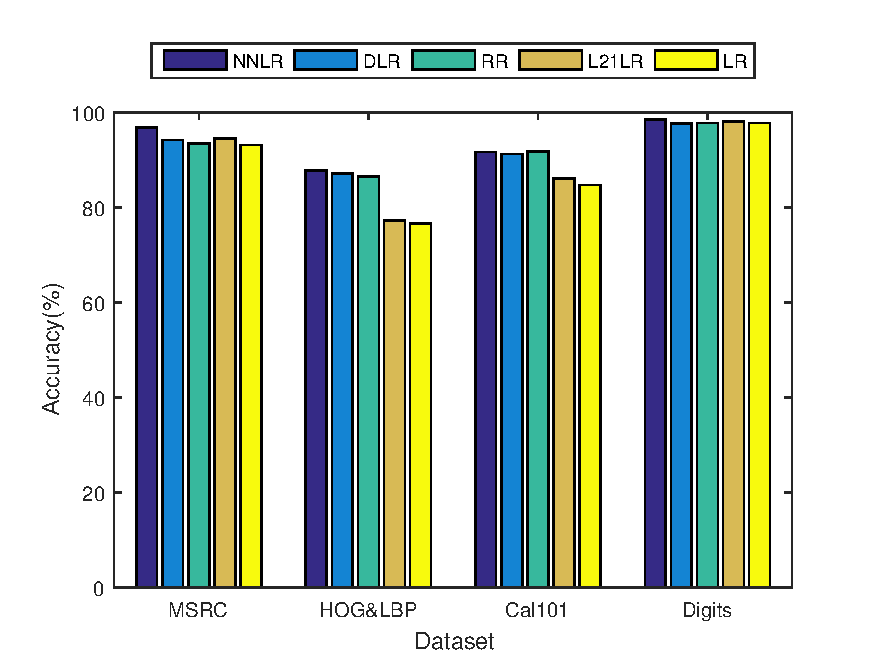
\includegraphics[width=8cm]{multi_view}\\
  \caption{Recognition rate of multi-view datasets.}\label{fig3}
\end{figure}




\begin{table*}[t]
\renewcommand\arraystretch{1.3}
\newcommand{\bb}[1]{\raisebox{0pt}[0pt][0pt]{\shortstack{#1}}}
\newcommand{\PreserveBackslash}[1]{\let\temp=\\#1\let\\=\temp}
\newcolumntype{C}[1]{>{\PreserveBackslash\centering}p{#1}}
\newcolumntype{R}[1]{>{\PreserveBackslash\raggedleft}p{#1}}
\newcolumntype{L}[1]{>{\PreserveBackslash\raggedright}p{#1}}
\caption{ Recognition rate of different methods on single-view datasets (mean$\pm$std\%).}\label{tab1}
\begin{center}
\begin{tabular}%{lccc}
{
C{40pt}
|@{\extracolsep{0.7pt}}C{60pt}@{\extracolsep{1pt}}
|@{\extracolsep{0.7pt}}C{60pt}@{\extracolsep{1pt}}
|@{\extracolsep{0.7pt}}C{60pt}@{\extracolsep{1pt}}
|@{\extracolsep{0.7pt}}C{60pt}@{\extracolsep{1pt}}
|@{\extracolsep{0.7pt}}C{60pt}@{\extracolsep{1pt}}
|@{\extracolsep{0.7pt}}C{60pt}@{\extracolsep{1pt}}}
\toprule
Dataset &AR &Extended Yale B  &Cal101-HOG & Cal101-LBP & Cal101-Sift & USPS\\
\hline
NNLR&\textbf{98.25$\pm$0.55}&\textbf{97.25$\pm$2.31}&\textbf{84.91$\pm$2.36}&\textbf{83.42$\pm$2.43} & \textbf{87.83$\pm$2.18} & \textbf{86.84$\pm$1.5}\\
\hline
LR-RR&98.11$\pm$0.61 & 96.45$\pm$2.67 & 83.60$\pm$2.43 & 82.05$\pm$2.40 & 87.27$\pm$2.25 & 84.15$\pm$1.65\\
 \hline
LR-ELM&97.52$\pm$2.78 & 95.75$\pm$2.78 & 79.44$\pm$2.55 & 76.34$\pm$3.13 & 80.93$\pm$3.19 & 82.28$\pm$2.15\\
 \hline
LRRR&97.68$\pm$0.67 & 96.55$\pm$2.42 & 83.73$\pm$2.23 & 82.48$\pm$2.36 & 86.89$\pm$2.02 & 85.93$\pm$1.5\\
 \hline
RR&  97.62$\pm$0.65 & 96.78$\pm$2.42 & 83.29$\pm$2.16 & 82.05$\pm$2.40 & 87.27$\pm$2.25 & 84.13$\pm$1.65\\
 \hline
L21LR& 91.98$\pm$9.22 & 72.82$\pm$3.11 & 65.90$\pm$11.01 & 80.06$\pm$3.82 & 86.65$\pm$2.18 & 77.71$\pm$2.85\\
 \hline
LR& 95.86$\pm$0.62 & 73.44$\pm$3.01 & 59.50$\pm$3.75 & 70.19$\pm$4.43 & 86.27$\pm$2.44 & 68.91$\pm$1.58\\
\toprule
\end{tabular}
\end{center}
\end{table*}


\begin{table*}[t]
\renewcommand\arraystretch{1.3}
\newcommand{\bb}[1]{\raisebox{0pt}[0pt][0pt]{\shortstack{#1}}}
\newcommand{\PreserveBackslash}[1]{\let\temp=\\#1\let\\=\temp}
\newcolumntype{C}[1]{>{\PreserveBackslash\centering}p{#1}}
\newcolumntype{R}[1]{>{\PreserveBackslash\raggedleft}p{#1}}
\newcolumntype{L}[1]{>{\PreserveBackslash\raggedright}p{#1}}
\caption{ Computing time of different methods on single-view datasets (mean$\pm$std\%).}\label{tab2}
\vspace{-2mm}
\begin{center}
\begin{tabular}%{lccc}
{
C{40pt}
|@{\extracolsep{0.7pt}}C{60pt}@{\extracolsep{1pt}}
|@{\extracolsep{0.7pt}}C{60pt}@{\extracolsep{1pt}}
|@{\extracolsep{0.7pt}}C{60pt}@{\extracolsep{1pt}}
|@{\extracolsep{0.7pt}}C{60pt}@{\extracolsep{1pt}}
|@{\extracolsep{0.7pt}}C{60pt}@{\extracolsep{1pt}}
|@{\extracolsep{0.7pt}}C{60pt}@{\extracolsep{1pt}}}
\toprule
Dataset & AR & Extended Yale B & Cal101-HOG & Cal101-LBP & Cal101-Sift & USPS\\
\hline
NNLR & 14.25$\pm$0.92 & 13.83$\pm$2.41 & 1.77$\pm$0.30 & 2.60$\pm$0.35 & 13.48$\pm$1.02 &0.63$\pm$0.07\\
\hline
LR-RR & 12.85$\pm$0.97 & 3.42$\pm$0.25 & 0.47$\pm$0.06 & 2.16$\pm$0.21 & 20.78$\pm$0.44 & 0.14$\pm$0.02\\
 \hline
LR-ELM & 35.8$\pm$2.91 & 34.87$\pm$1.85 & 0.79$\pm$0.03 & 11.14$\pm$0.36 & 10.13$\pm$0.62 & 14.50$\pm$1.76\\
 \hline
LRRR& 27.21$\pm$1.29 & 3.11$\pm$0.16 & 0.59$\pm$0.03 & 2.96$\pm$0.17 & 27.35$\pm$6.79 & 0.14$\pm$0.02\\
 \hline
RR&  21.90$\pm$0.87 & 3.54$\pm$0.33 & 0.59$\pm$0.08 & 3.64$\pm$0.44 & 34.14$\pm$3.08 & 0.06$\pm$0.01\\
 \hline
L21LR&129.55$\pm$23.46 &3.61$\pm$0.32 &7.72$\pm$1.01 &71.24$\pm$3.78 & 566.2$\pm$19.32 & 2.50$\pm$0.24\\
 \hline
LR&13.68$\pm$1.23 &2.88$\pm$0.22 & 0.34$\pm$0.04 & 2.50$\pm$0.22 & 26.17$\pm$2.30 & 0.07$\pm$0.02\\
\toprule
\end{tabular}
\end{center}
\vspace{-4mm}
\end{table*}

\begin{table*}[!t]
\renewcommand\arraystretch{1.3}
\newcommand{\bb}[1]{\raisebox{0pt}[0pt][0pt]{\shortstack{#1}}}
\newcommand{\PreserveBackslash}[1]{\let\temp=\\#1\let\\=\temp}
\newcolumntype{C}[1]{>{\PreserveBackslash\centering}p{#1}}
\newcolumntype{R}[1]{>{\PreserveBackslash\raggedleft}p{#1}}
\newcolumntype{L}[1]{>{\PreserveBackslash\raggedright}p{#1}}
\caption{  Recognition rate of different methods on multi-view datasets (mean$\pm$std\%).}\label{tab3}
\begin{center}
\begin{tabular}%{lccc}
{
C{50pt}
%|@{\extracolsep{0.7pt}}C{52pt}@{\extracolsep{1pt}}
%|@{\extracolsep{0.7pt}}C{50pt}@{\extracolsep{1pt}}
|@{\extracolsep{0.7pt}}C{70pt}@{\extracolsep{1pt}}
|@{\extracolsep{0.7pt}}C{70pt}@{\extracolsep{1pt}}
|@{\extracolsep{0.7pt}}C{70pt}@{\extracolsep{1pt}}
|@{\extracolsep{0.7pt}}C{70pt}@{\extracolsep{1pt}}}
\toprule
 Dataset &  MSRC & Cal101-HOG\&LBP & Cal101 & Digits\\
 \hline
NNLR &\textbf{ 96.76$\pm$1.75} & \textbf{87.76$\pm$1.31} & 91.68$\pm$1.50 & \textbf{98.42$\pm$0.15}\\
  \hline
LRRR & 94.19$\pm$2.52 & 87.08$\pm$1.16 & 91.24$\pm$1.46 & 97.61$\pm$0.23\\
  \hline
RR & 93.43$\pm$2.99 & 86.46$\pm$1.24 & \textbf{91.74$\pm$1.00} & 97.69$\pm$0.17\\
  \hline
L21LR & 94.48$\pm$2.05 & 77.2$\pm$8.56 & 86.09$\pm$5.67 & 98.02$\pm$0.24\\
  \hline
LR & 93.14$\pm$2.72 & 76.58$\pm$3.18 & 84.66$\pm$3.32 & 97.72$\pm$0.19\\
\toprule
\end{tabular}
\end{center}
\end{table*}


\begin{table*}[!t]
\renewcommand\arraystretch{1.3}
\newcommand{\bb}[1]{\raisebox{0pt}[0pt][0pt]{\shortstack{#1}}}
\newcommand{\PreserveBackslash}[1]{\let\temp=\\#1\let\\=\temp}
\newcolumntype{C}[1]{>{\PreserveBackslash\centering}p{#1}}
\newcolumntype{R}[1]{>{\PreserveBackslash\raggedleft}p{#1}}
\newcolumntype{L}[1]{>{\PreserveBackslash\raggedright}p{#1}}
\caption{  Computing time of different methods on multi-view datasets (mean$\pm$std\%).}\label{tab4}
\begin{center}
\begin{tabular}%{lccc}
{
C{50pt}
%|@{\extracolsep{0.7pt}}C{52pt}@{\extracolsep{1pt}}
%|@{\extracolsep{0.7pt}}C{50pt}@{\extracolsep{1pt}}
|@{\extracolsep{0.7pt}}C{70pt}@{\extracolsep{1pt}}
|@{\extracolsep{0.7pt}}C{70pt}@{\extracolsep{1pt}}
|@{\extracolsep{0.7pt}}C{70pt}@{\extracolsep{1pt}}
|@{\extracolsep{0.7pt}}C{70pt}@{\extracolsep{1pt}}}
\toprule
 Dataset &  MSRC & Cal101-HOG\&LBP & Cal101 & Digits\\
 \hline
NNLR &\textbf{ 0.21$\pm$0.04} & 6.77$\pm$0.43 &\textbf{ 6.63$\pm$0.54} & 0.63$\pm$0.09\\
  \hline
LRRR & 8.56$\pm$0.55 & 15.06$\pm$0.46 & 282$\pm$47.02 & 0.87$\pm$0.08\\
  \hline
RR & 1.78$\pm$0.20 & 4.21$\pm$0.16 & 35.5$\pm$2.03 & 0.12$\pm$0.01\\
  \hline
L21LR &  4.08$\pm$0.23 & 73.85$\pm$1.51 & 848.98$\pm$25.18 & 1.73$\pm$0.23\\
  \hline
LR & 0.55$\pm$0.04 & \textbf{3$\pm$0.24} & 25.88$\pm$2.14 & \textbf{0.05$\pm$0.01}\\
\toprule
\end{tabular}
\end{center}
\end{table*}

\subsection{Multi-view Experiments}
Previous work~\cite{ref19,ref25} show that ridge regression will have better performance than linear regression. However, all existing work is based on a single view. Does multi-view ridge regression produce better results than multi-view linear regression? Therefore, we will examine the performance of all methods on multi-view datasets.

We use 4 datasets in the multi-view experiment, which are MSRC, Digits, Cal101(using 3 features as 3 views respectively) and Cal101-HOG\&LBP (using Cal101-HOG and Cal101-LBP of Cal101 as 2 views respectively). Summary of the datasets attributes are presented in TABLE \ref{tab6}, where $n$ is sample number, $c$ is class number, $v$ is view number and $d_v$ lists the dimensions of different views. For Digits and MSRC, 50\% images of each individual randomly selected are used as the training set and the rest as the testing set. For cal101 and Cal101-HOG\&LBP dataset, we randomly select 290 images for training and the rest for test. Similarly, we computed the training time (in seconds) of all the methods on the datasets.

To help researchers easily compare the efficiency of two kind low rank regression method, we define a variable $r$,
\begin{equation}\label{eq21}
r = \frac{{{t_{LRRR}}}}{{{t_{NNLR}}}}
\end{equation}
\noindent where ${{t_{LRRR}}}$ is the training time of LRRR and ${{t_{NNLR}}}$ is the training time of NNLR. We use the training time of NNLR and LRRR on Cal101-HOG, Cal101-LBP, Cal101-Sift, Cal101-HOG\&LBP and Cal101 to calculate $r$ and plot the curve of $r$ versus dimension of those datasets. The curve is showed in FIGURE \ref{fig4}. In addition, FIGURE \ref{fig3} shows that the recognition rate histogram, TABLE \ref{tab3} shows the mean and standard deviation of accuracy over 10 random splits. TABLE \ref{tab3} describes the mean and standard deviation of computing time.



\begin{figure}[t]
  \centering
  % Requires \usepackage{graphicx}
  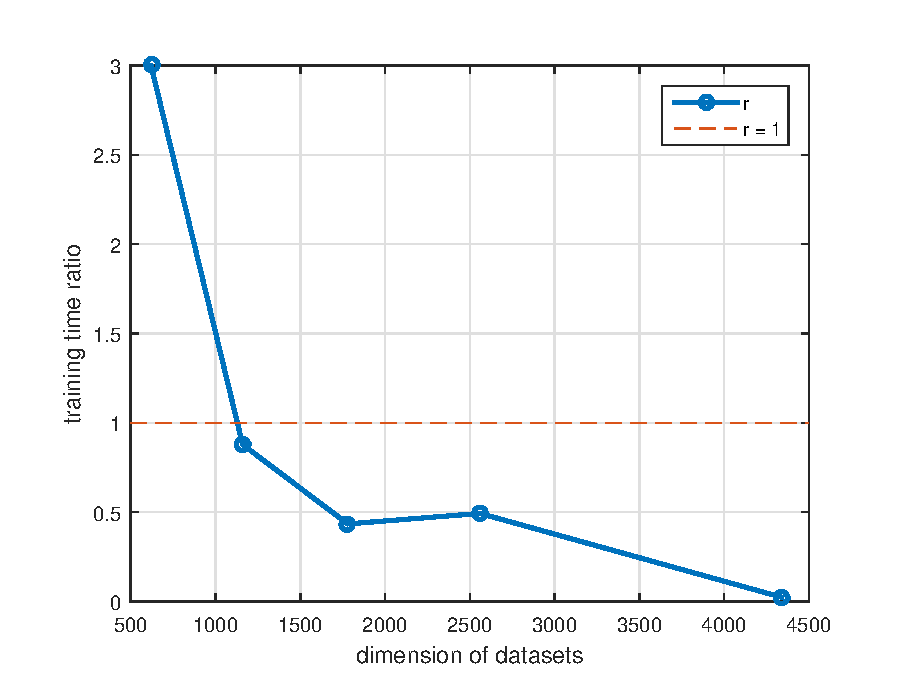
\includegraphics[width=8cm]{dimension_time}\\
  \caption{The curve of $r$ versus dimension.}\label{fig4}
\end{figure}

\begin{figure}[t]
  \centering
  % Requires \usepackage{graphicx}
  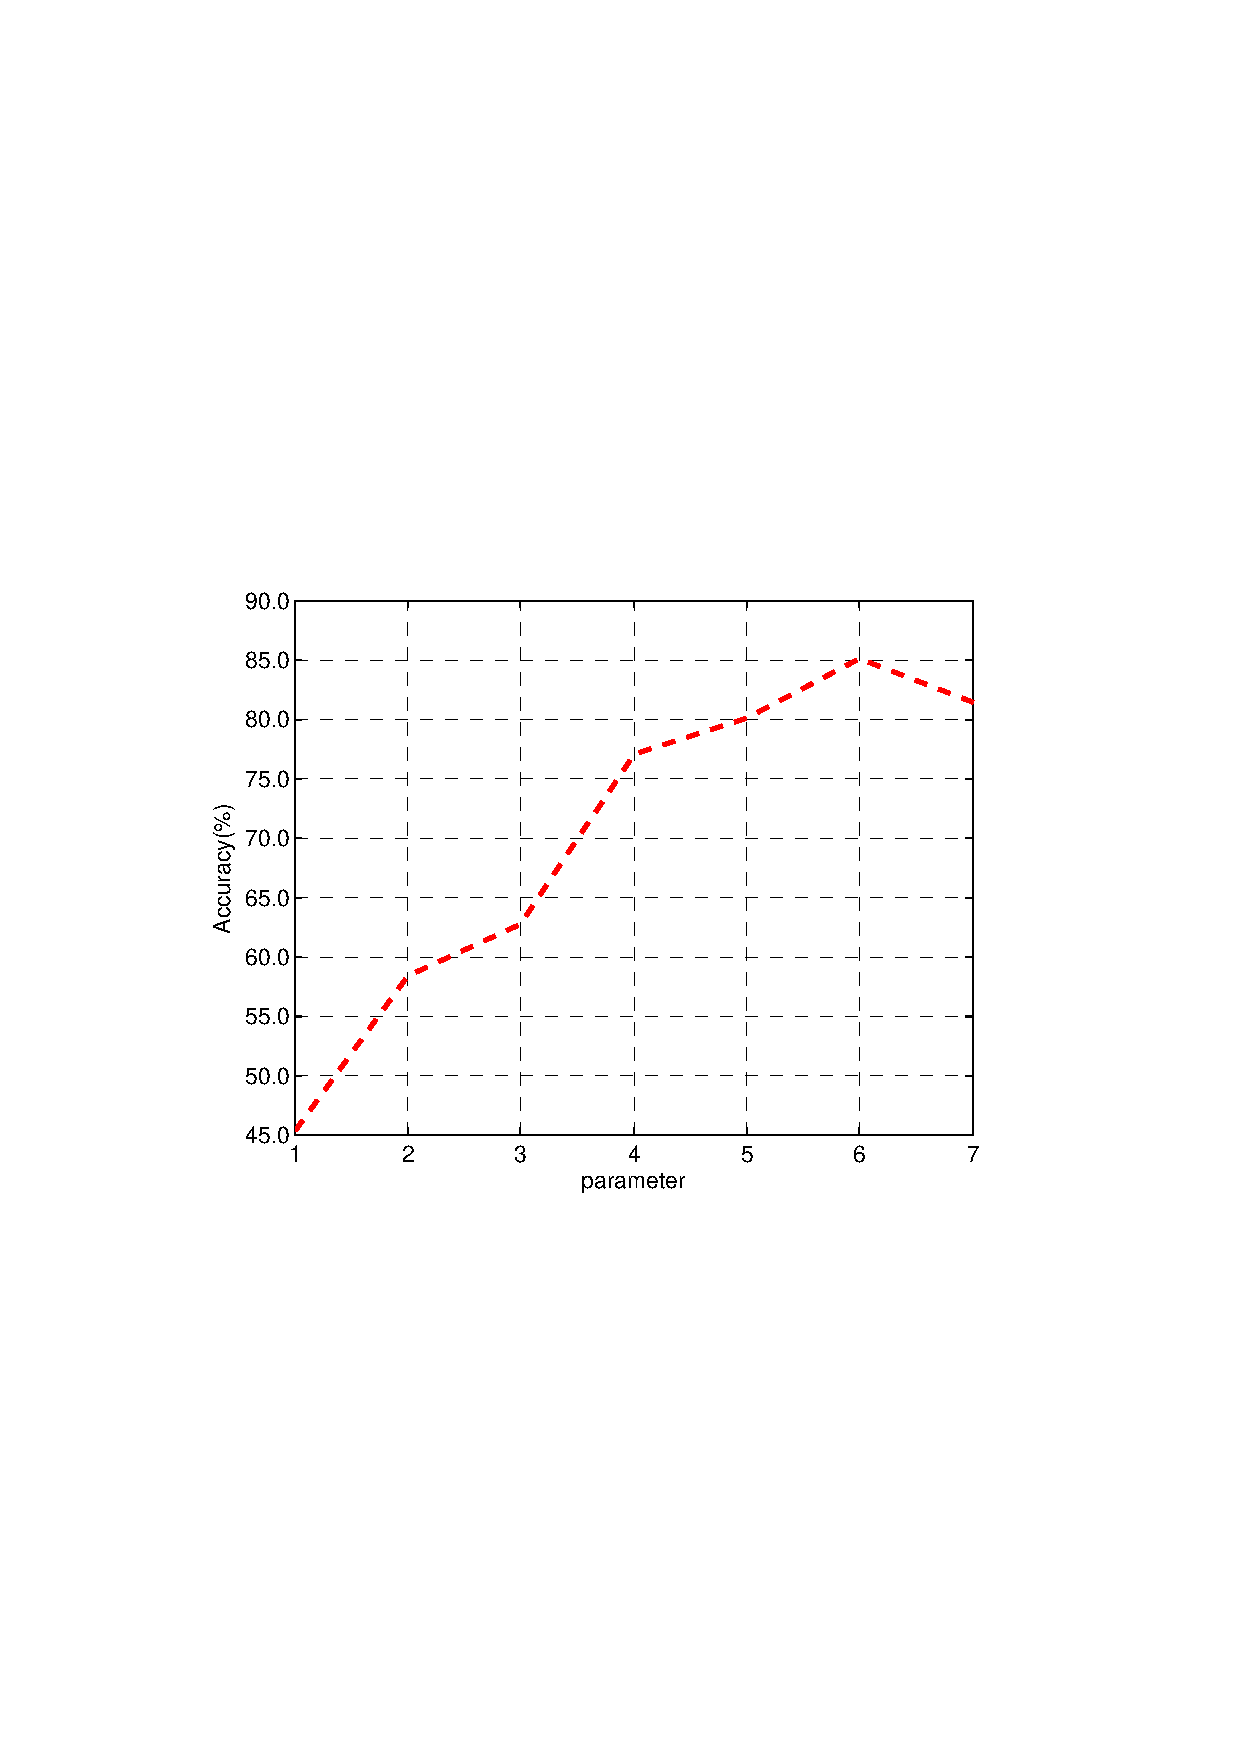
\includegraphics[width=8cm]{lrrr_para}\\
  \caption{Recognition rate of lRRR with different parameters of low rank constraints.}\label{fig9}
\end{figure}

\begin{figure*}[t]
  \centering
  % Requires \usepackage{graphicx}
  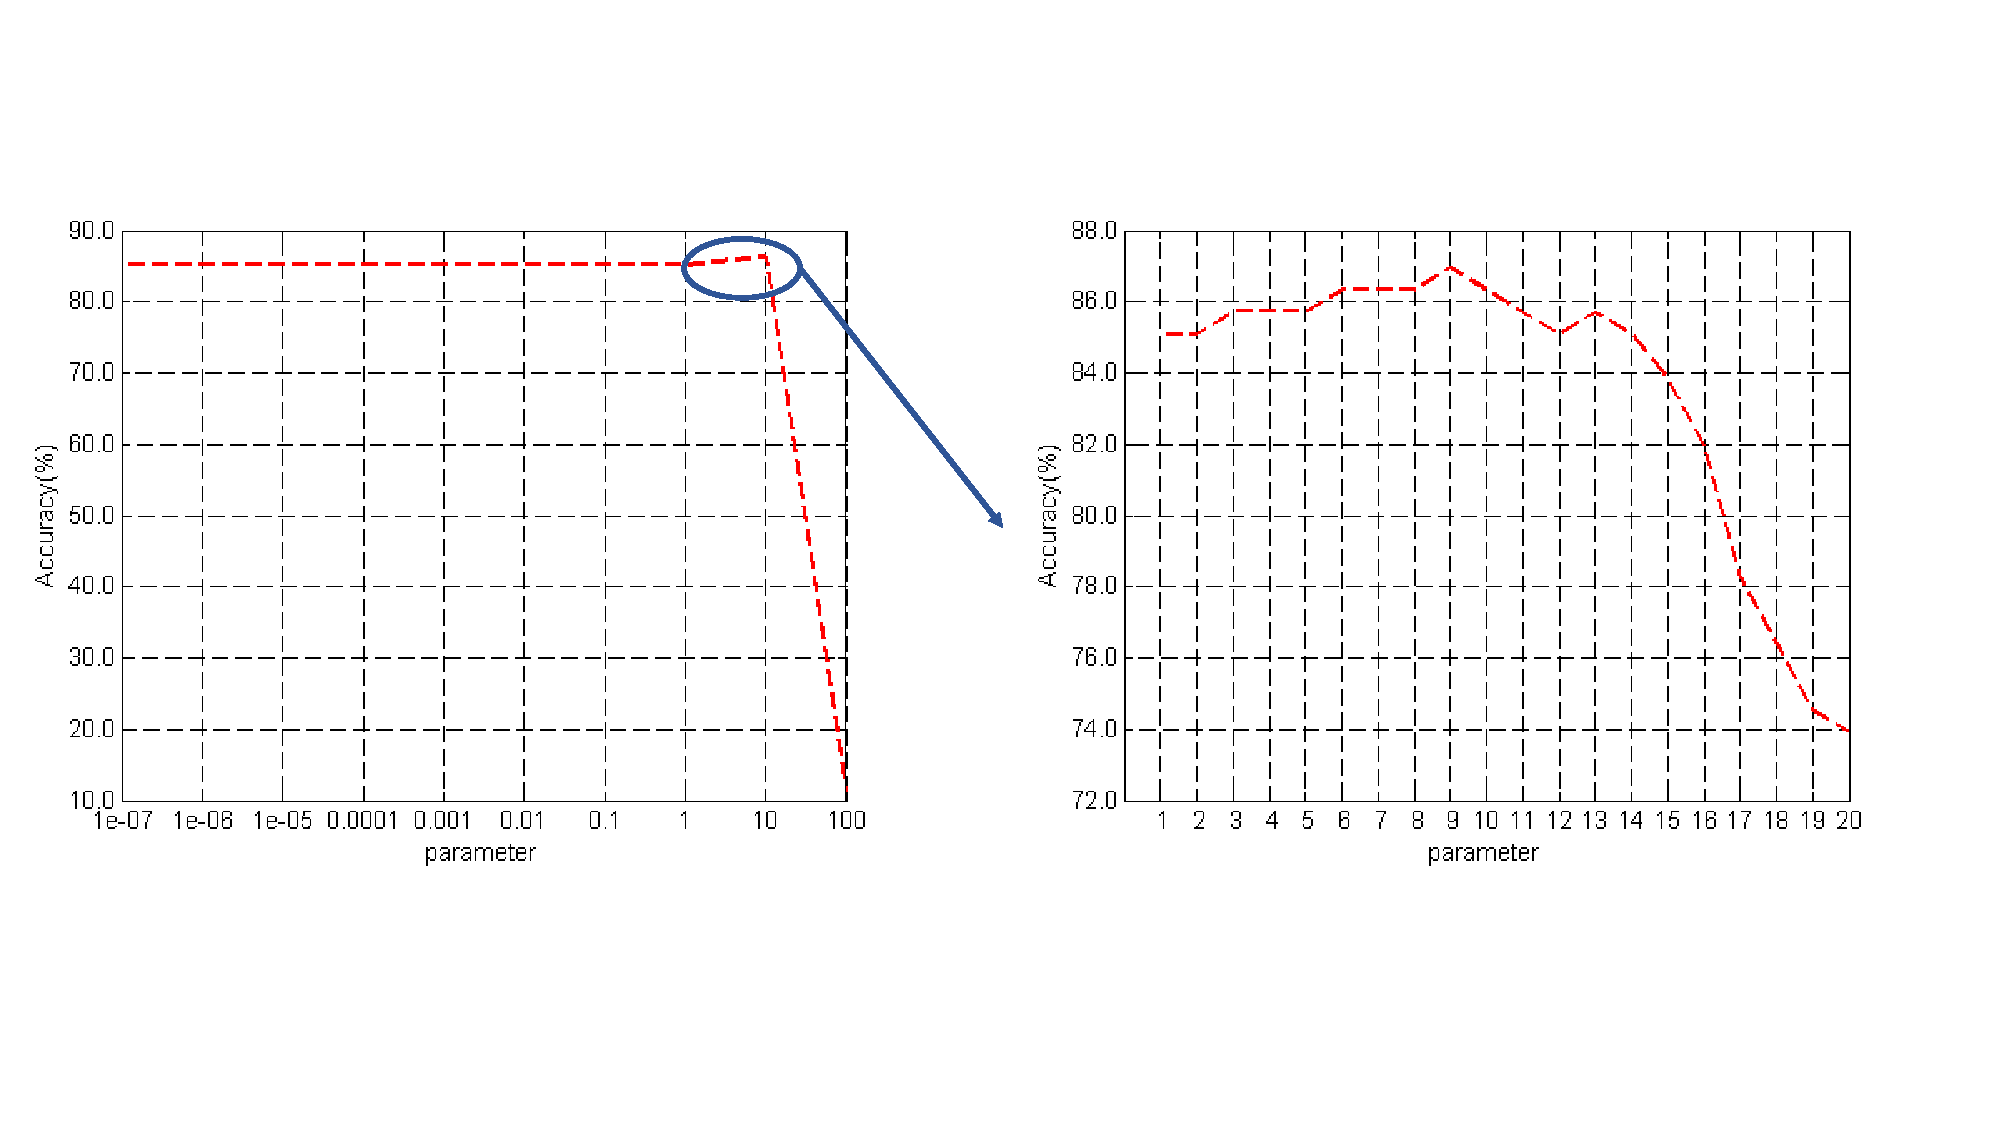
\includegraphics[width=17cm]{nnlr_para}\\
  \caption{Recognition rate of NNLR with different parameters of low rank constraints.}\label{fig10}
\end{figure*}


\subsection{Experiment results and analysis}
From FIGURE \ref{fig2}, FIGURE \ref{fig3} and TABLE \ref{tab1}, TABLE \ref{tab2}, we can obtain some interesting observations.

\begin{enumerate}
  \item \textbf{Comparison of linear regression(LR) and the regularized linear regression methods.} The regularized linear regression methods achieve better recognition rate than LR in single-view datasets and multi-view datasets. FIGURE \ref{fig2} and TABLE \ref{tab1} show that NNLR, LR-RR, LR-ELM, LRRR and RR produce better recognition rate than LR in all single-view datasets, L21LR outperforms LR in single-view datasets Cal101 and USPS. FIGURE \ref{fig3} and TABLE \ref{tab2} show that all the regularized linear regression methods have better recognition rate than LR in all multi-view datasets. The reason is that those regularized method provide priori constraints on the coefficient matrix and improve the discriminant ability of methods. This indicates that regularization item plays an important role in enhancing the performance of linear regression.
  \item \textbf{Comparison with other low-rank regularized regression methods.} Both LRRR and NNLR are based on ridge regression, and they explore the low rank structure of data and alleviate the rank deficiency problem.  In addition, NNLR takes into account the global geometric structure which described by nuclear norm of projected data. FIGURE \ref{fig2}, FIGURE \ref{fig3} and TABLE \ref{tab1}, TABLE \ref{tab2} show that NNLR has better recognition rate than LRRR in all single-view datasets and all multi-view datasets. This indicates that preserve global geometric structure is useful to improve the discriminant capability of feature decreased dimension and enhance the learning model.

      From TABLE \ref{tab1}, we can see LR-RR achieves lower performance than NNLR and LRRR. The reason may be that LR-RR is mainly focus on the case that the data is `dirty', i.e. data has much noise. When the data is clean, its performance degenerate to RR.
  \item \textbf{Comparison of sigle-view methods and multi-view methods.} Multi-view regression methods use data or information from multiple channels, such as different image features, both webpage citations view and contents view. Generally, we expect
that multi-view regression can produce better results by exploiting information from multiple views. TABLE \ref{tab1} and TABLE \ref{tab2} show that the results of all single-view methods in sigle-view datasets Cal101-HOG and Cal101-LBP is lower than the results of multi-view methods in multi-view datasets Cal101-HOG\&LBP and Cal101, the results of all single-view methods in sigle-view datasets Cal101-HOG, Cal101-HOG and Cal101-sift is lower than the results of multi-view methods in multi-view dataset Cal101. The reason is that Cal101-HOG\&LBP and Cal101 have much more view data and provide more useful information. The multi-view method in our experiment can be seen as an ensemble of single-view method on single-view data. As a result, it has better accuracy than single-view methods.
  \item \textbf{Comparison of computing time of different methods.} The computing time of different methods are showed in TABLE \ref{tab2} and \ref{tab4}. FIGURE \ref{fig4} shows the training time ratio of NNLR to LRRR versus dimension of data. From which, we can find that when there is increasing dimension of data, training time of NNLR is less than LRRR. The reason is that when the dimension of data is big and the number of samples in dataset is approximate, the computation complexity is mainly affected by data dimension $p$. Ignoring other variables, the computational cost of NNLR and LRRR can be simplified as $o(p)$ and $o({p^2})$, which is consistent with FIGURE \ref{fig4}. There is a prerequisite for this conclusion that the number of samples is small. Therefore, when there are small samples and large dimension, NNLR gets higher recognition rate and lower uses less computing time.

  \item \textbf{Comparison of bias-variance trade-off in the model fitting} LRRR solves the low rank regression problem by using  matrix decomposition. Compared to the discontinuous LRRR, the proposed method NNLR results in a continuous solution path and allows a more flexible bias-variance trade-off in model fitting. FIGURE \ref{fig9} and \ref{fig10} show the recognition rate of NNLR and LRRR with different parameters of low rank constraints in dataset Col101-HOG, we can found that NNLR has larger adjustment range for model fitting, which results more flexible bias-variance trade-off.
  %\item From TABLE \ref{tab1}, we can see LR-RR achieves lower performance than NNLR and LRRR. The reason may be that LR-RR is mainly focus on the case that the data is `dirty', i.e. data has much noise. When the data is clean, its performance degenerate to RR.
\end{enumerate}

Thus, our newly proposed NNLR method are efficient and practical low rank method for machine learning applications.

\section{Conclusion}

In this paper, we proposed a novel low rank regression named NNLR. NNLR uses a nuclear norm item of the product of the data matrix and the coefficient matrix to explore the low rank structure of data based on ridge regression. Since there is no closed form solution to the optimization problem, we design an iterative algorithm to solve the optimal problem. Compared to classical method and related method such as LRRR and L21LR, we perform extensive experiment on some well-known dataset, from which we can find that NNLR has the best performance. For the dataset that the dimension is large and the number is small, NNLR has less computing-time consumption than LRRR which has a closed form solution��However, this advantage will not be maintained when the number of sample is large��overcoming this limitations will be our future work.


\section*{Acknowledgment}


%{\small
%\bibliographystyle{ieee}
%
%\bibliography{egbib}

\bibliographystyle{IEEEtran}
\bibliography{ompca_ref}

%\begin{IEEEbiography}[{\includegraphics[width=1in,height=1.25in,clip,keepaspectratio]{a2.png}}]{First A. Author} (M'76--SM'81--F'87) and all authors may include
%biographies. Biographies are often not included in conference-related
%papers. This author became a Member (M) of IEEE in 1976, a Senior
%Member (SM) in 1981, and a Fellow (F) in 1987. The first paragraph may
%contain a place and/or date of birth (list place, then date). Next,
%the author's educational background is listed. The degrees should be
%listed with type of degree in what field, which institution, city,
%state, and country, and year the degree was earned. The author's major
%field of study should be lower-cased.
%
%The second paragraph uses the pronoun of the person (he or she) and not the
%author's last name. It lists military and work experience, including summer
%and fellowship jobs. Job titles are capitalized. The current job must have a
%location; previous positions may be listed
%without one. Information concerning previous publications may be included.
%Try not to list more than three books or published articles. The format for
%listing publishers of a book within the biography is: title of book
%(publisher name, year) similar to a reference. Current and previous research
%interests end the paragraph. The third paragraph begins with the author's
%title and last name (e.g., Dr.\ Smith, Prof.\ Jones, Mr.\ Kajor, Ms.\ Hunter).
%List any memberships in professional societies other than the IEEE. Finally,
%list any awards and work for IEEE committees and publications. If a
%photograph is provided, it should be of good quality, and
%professional-looking. Following are two examples of an author's biography.
%\end{IEEEbiography}
%
%\begin{IEEEbiography}[{\includegraphics[width=1in,height=1.25in,clip,keepaspectratio]{a2.png}}]{Second B. Author} was born in Greenwich Village, New York, NY, USA in
%1977. He received the B.S. and M.S. degrees in aerospace engineering from
%the University of Virginia, Charlottesville, in 2001 and the Ph.D. degree in
%mechanical engineering from Drexel University, Philadelphia, PA, in 2008.
%
%From 2001 to 2004, he was a Research Assistant with the Princeton Plasma
%Physics Laboratory. Since 2009, he has been an Assistant Professor with the
%Mechanical Engineering Department, Texas A{\&}M University, College Station.
%He is the author of three books, more than 150 articles, and more than 70
%inventions. His research interests include high-pressure and high-density
%nonthermal plasma discharge processes and applications, microscale plasma
%discharges, discharges in liquids, spectroscopic diagnostics, plasma
%propulsion, and innovation plasma applications. He is an Associate Editor of
%the journal \emph{Earth, Moon, Planets}, and holds two patents.
%
%Dr. Author was a recipient of the International Association of Geomagnetism
%and Aeronomy Young Scientist Award for Excellence in 2008, and the IEEE
%Electromagnetic Compatibility Society Best Symposium Paper Award in 2011.
%\end{IEEEbiography}



\EOD

\end{document}
